\documentclass[11pt,a4paper]{report}
\usepackage{marvosym}

\assignment{2}
\group{1 (Moodle), 39 (INGInious)}
\students{Victor Carballes Cordoba (NOMA : 34472100)}{Krystian Targonski (NOMA : 42942000)}

\begin{document}

\maketitle

Answer to the questions by adding text in the boxes. You may answer in either \textbf{French or English}. Do not modify anything else in the template.  The size of the boxes indicate the place you \textbf{can} use, but you \textbf{need not} use all of it (it is not an indication of any expected length of answer). \textbf{Be as concise as possible! A good short answer is better than a lot of nonsense!}
%\bigskip

\section{Exercises (5~pts)}

\textit{The following figure assigns a unique letter to each node, and a unique number to each branch. Use it to answer the following questions.}
\begin{center}
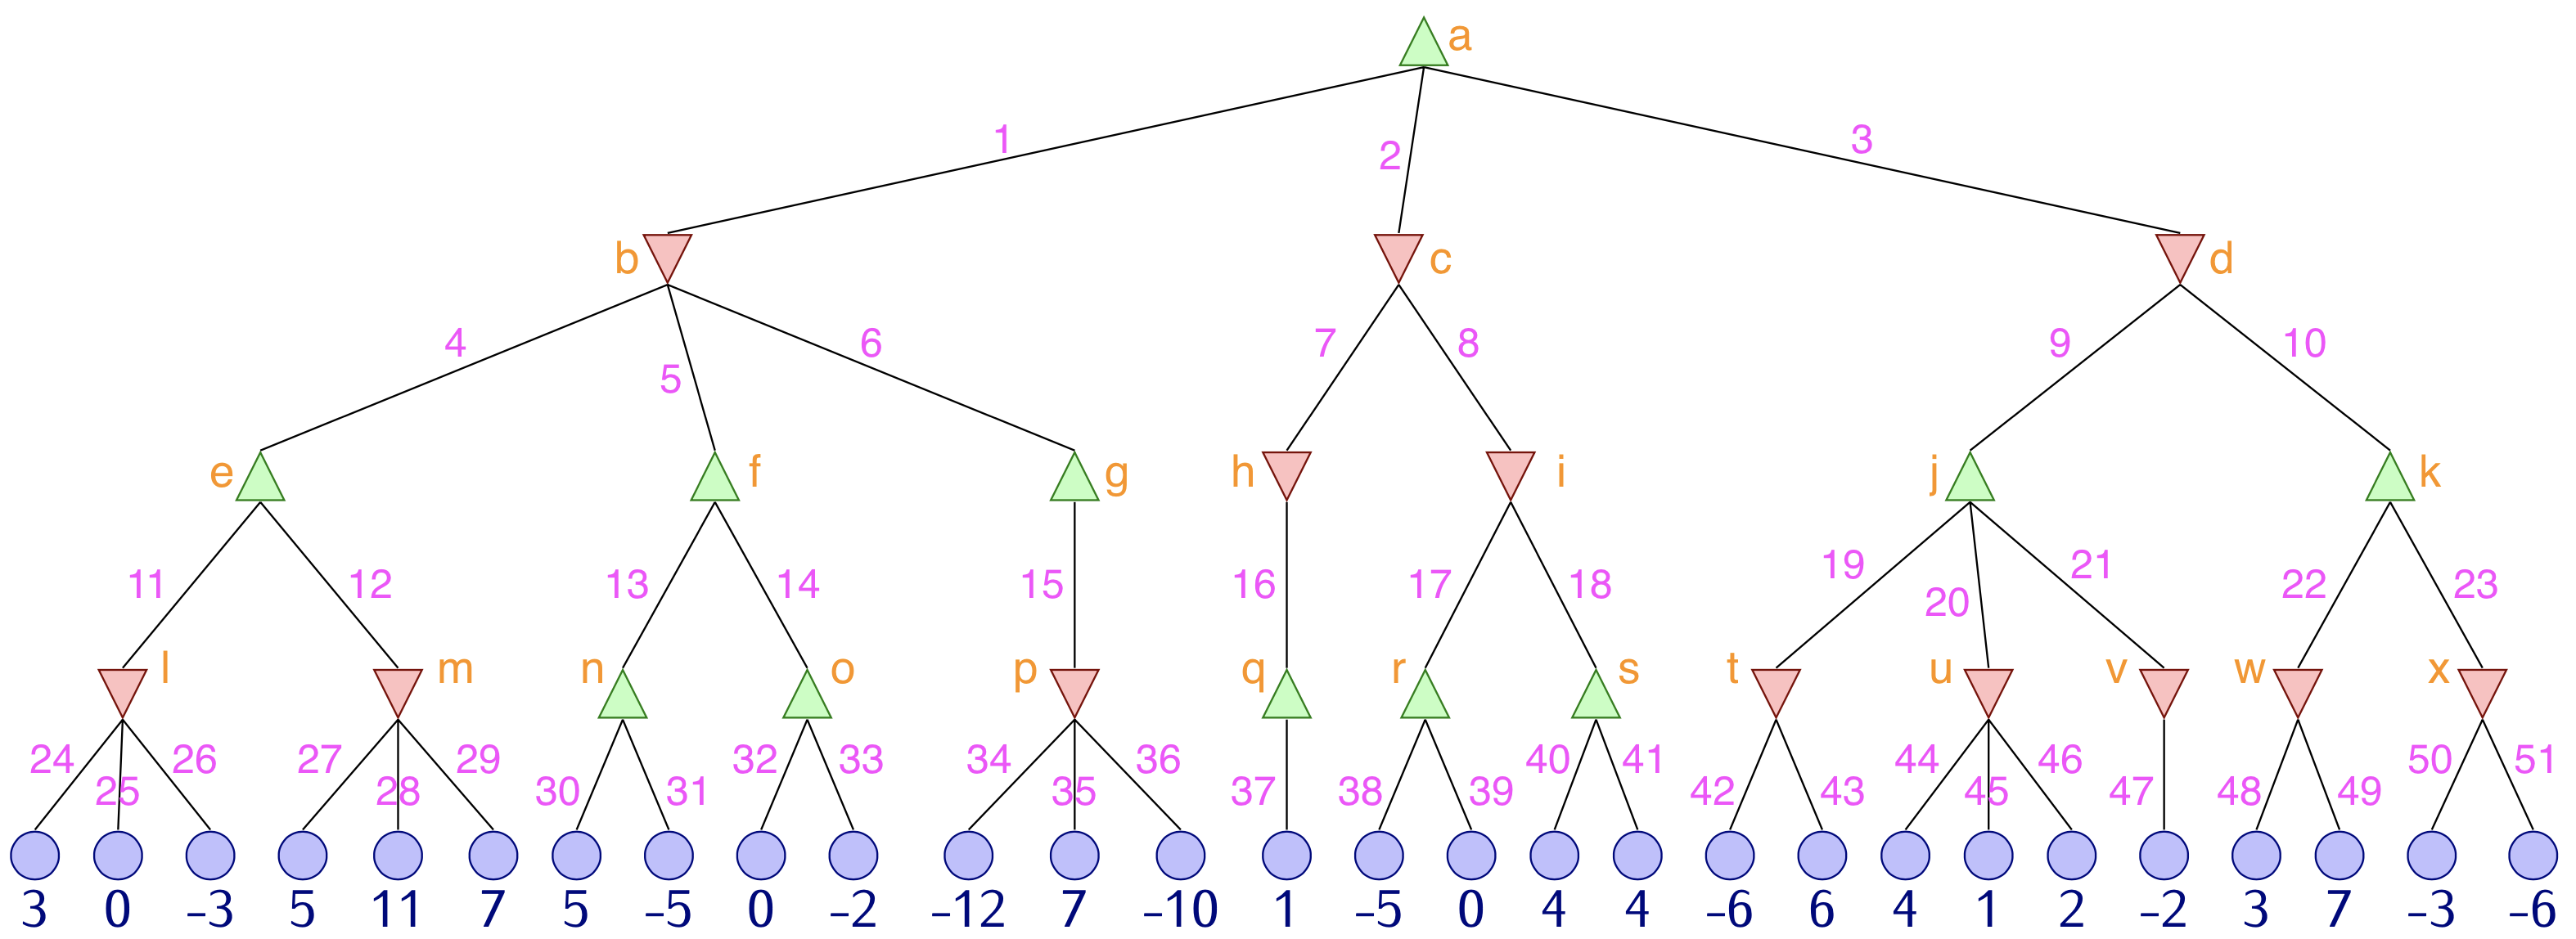
\includegraphics[width=\linewidth]{images/minimax_labelled.png}
\end{center}


\begin{enumerate}
\item Perform the MiniMax algorithm on the following tree, i.e.
      put a value to each node. What move should the root player do? \textbf{(1~pt)}
      
      \textit{Assign a numerical value to each node, and indicate the move (i.e.\! 1, 2, or 3) to perform:}
\end{enumerate}
      \begin{answers}[3cm]
      \begin{multicols}{5}
      \textbf{a: 1} %TODO Insert your answer here
      
      \textbf{b: -12} %TODO Insert your answer here
      
      \textbf{c: 0} %TODO etc.
      
      \textbf{d: 1}
      
      \textbf{e: 5}
      
      \textbf{f: 5}
      
      \textbf{g: -12}
      
      \textbf{h: 1}
      
      \textbf{i: 0}
      
      \textbf{j: 1}
      
      \textbf{k: 3}
      
      \textbf{l: -3}
      
      \textbf{m: 5}
      
      \textbf{n: 5}
      
      \textbf{o: 0}
      
      \textbf{p: -12}
      
      \textbf{q: 1}
      
      \textbf{r: 0}
      
      \textbf{s: 4}
      
      \textbf{t: -6}
      
      \textbf{u: 1}
      
      \textbf{v: -2}
      
      \textbf{w: 3}
      
      \textbf{x: -6}
      
      \textbf{Move: 3} %TODO Insert 1, 2 or 3 here
      \end{multicols}
	  \end{answers}



\begin{enumerate}
\item[2.] Perform the Alpha-Beta algorithm on the same tree.
      At each non terminal node, put the successive values of $\alpha$ and
      $\beta$. Cross out the arcs reaching non visited nodes. Assume a
      left-to-right node expansion. \textbf{(1~pt)}
      
      \textit{Indicate the successive $\alpha$ and $\beta$ values of each node in the table below. Separate successive values by a comma (,). Indicate at the bottom the identifiers of the branches that are cut (in increasing order, separated by a comma) (indicate only the branches where the cuts happen, i.e.\!} don't \textit{indicate the branches that are below a cut).}
\end{enumerate}

\begin{answers}[8cm]
    \begin{multicols}{2}
    \begin{tabular}{ccc}
    Node & $\alpha$ values & $\beta$ values\\
    \hline
    \textbf{a} &-inf,-12,0,1  &inf,1 \\ %TODO Insert your answer in the table (example: \textbf{a} & 1, 3, 2 & 5, 4 \\)
    \textbf{b} &-inf,-12  &inf,5,-12  \\
    \textbf{c} &-inf,0  &inf,1,0  \\
    \textbf{d} &-inf,1  &inf,1  \\
    \textbf{e} &-inf,-3,5 &inf,5  \\
    \textbf{f} &-inf,5  &inf  \\
    \textbf{g} &-inf,-12  &inf,-12  \\
    \textbf{h} &-inf,1  &inf,1  \\
    \textbf{i} &-inf,0  &inf,0  \\
    \textbf{j} &-inf,-6,1  &inf,1  \\
    \textbf{k} &-inf,3  &inf  \\
    \textbf{l} &-inf,-3  &3,0,-3  \\
    \textbf{m} &-inf,5  &5  \\ 
    \end{tabular}
    
    \begin{tabular}{ccc}
    Node & $\alpha$ values & $\beta$ values\\
    \hline
    \textbf{n} &5  &inf,5  \\
    \textbf{o} &/  &/  \\
    \textbf{p} &-inf,12  &-12  \\
    \textbf{q} &1  &1  \\
    \textbf{r} &-5,0  &inf,0  \\
    \textbf{s} &4  &inf,4  \\
    \textbf{t} &-inf,-6  &-6  \\
    \textbf{u} &-inf,1  &4,1  \\
    \textbf{v} &-2  &-2  \\
    \textbf{w} &-inf,3  &3  \\
    \textbf{x} &/  &/  \\
     &  &  \\
    \end{tabular}
    \end{multicols}
    
\textbf{Cuts: 14, 51} %TODO Insert your answer here (example: 2, 4, 6, 8, 10)
\end{answers}





\begin{enumerate}
\item[3.] Do the same, assuming a right-to-left node expansion instead.  \textbf{(1~pt)}
\end{enumerate}

\begin{answers}[8cm]
      \begin{multicols}{2}
      \begin{tabular}{ccc}
      Node & $\alpha$ values & $\beta$ values\\
      \hline
      \textbf{a} &-inf,1 &inf \\ %TODO Insert your answer in the table (example: \textbf{a} & 1, 3, 2 & 5, 4 \\)
      \textbf{b} &-inf  &inf,-12  \\
      \textbf{c} &-inf  &inf,0  \\
      \textbf{d} &-inf,1  &inf,3,1  \\
      \textbf{e} &/  &/  \\
      \textbf{f} &/  &/  \\
      \textbf{g} &-inf,-12  &inf,-12  \\
      \textbf{h} &/  &/  \\
      \textbf{i} &-inf,0  &inf,4,0  \\
      \textbf{j} &-inf,-2,1  &inf,1  \\
      \textbf{k} &-inf,-6,3  &inf,3  \\
      \textbf{l} &/  &/  \\
      \textbf{m} &/  &/  \\ 
      \end{tabular}
      
      \begin{tabular}{ccc}
      Node & $\alpha$ values & $\beta$ values\\
      \hline
      \textbf{n} &/  &/  \\
      \textbf{o} &/  &/  \\
      \textbf{p} &-inf,-12  &-10,-12  \\
      \textbf{q} &/  &/  \\
      \textbf{r} &0  &inf,0  \\
      \textbf{s} &4  &inf,4  \\
      \textbf{t} &-inf,-6  &6,-6  \\
      \textbf{u} &-inf,1  &2,1  \\
      \textbf{v} &-2  &-2  \\
      \textbf{w} &-inf,3  &7,3  \\
      \textbf{x} &-inf,-6  &-6  \\
       &  &  \\
      \end{tabular}
      \end{multicols}
      
\textbf{Cuts: 4, 5, 7} %TODO Insert your answer here (example: 2, 4, 6, 8, 10)
\end{answers}




\clearpage
\begin{enumerate}
\item[4.] Is there a node ordering that can lead to a more optimal pruning of the tree
(in the sense where the algorithm prunes more branches than in the two other
considered cases)? If no, explain why. If yes, give a new node ordering and the
resulting new pruning.  \textbf{(1~pt)}
      
      \textit{Insert an image below containing the reordered tree, with successive $\alpha$/$\beta$ values indicated next to each node, and where the branches that are cut by the algorithm are crossed out. This may either be an edited version of \texttt{minimax\_empty.png} (using paint, gimp, etc.), a photograph of a drawing you made by hand, etc. In any case, the image must be \textbf{clear} in order to be graded.}
\end{enumerate}

\begin{answers}[8cm]
%TODO Insert the path to your image between the {}. 
% Possibly adjust the scale parameter so your image fits in the box.
%\includegraphics[scale=.3]{...}
Yes there is, we can prune a bit more by ordering the nodes in this way and having a right-to-left node expansion
\end{answers}




\begin{enumerate}
\item[5.] How does Alpha-Beta need to be modified for games with more than two players? \textbf{(1~pt)}
\end{enumerate}

\begin{answers}[9cm]
%TODO Insert your answer here
pour minmax utility -> vecteur de plusieurs valeurs 
une fois qu'on a le vecteur -> chaque joueur à son tour prends l'action la plus efficace pour lui
\end{answers}





\clearpage
\section{Shobu (35~pts)}
\medskip

\subsection{Alpha-Beta agent (4 points, to be submitted on Inginious)}
\medskip


\subsection{Monte-Carlo Tree Search agent (5 points, to be submitted on Inginious)}
\medskip


\subsection{Warm-up questions (3 points)}
\begin{enumerate}
\item[1.] What is the branching factor at the start of the game? What is the mean empirical branching factor? (The branching factor is considered here as the number of possible moves that a player can do from a given state). \textbf{(1 point)}
\end{enumerate}

\begin{answers}[5cm]
    % TODO put your answer here
    First off, we would like to mention that we counted an "action" as a single piece moving, in other words, passive and active moves are both counted ! 
    In the case where no one has moved yet and our definition of an action, the branching factor is 18*6 = 108.
\end{answers}



\begin{enumerate}
\item[2.] What would be one (of the many) drawbacks of the simple heuristic that is imposed for the basic alpha-beta agent above? \textbf{(1 point)}
\end{enumerate}

\begin{answers}[10cm]
    % TODO put your answer here
    Whenever the agent can clearly take an opponent's piece out, it does not always do it if the heuristic is kept simple
\end{answers}



\begin{enumerate}
\item[3.] Considering the Monte-Carlo Tree Search algorithm, what is the hypothesis supporting the use of random simulation to estimate the win rate? Is this hypothesis always valid? \textbf{(1 point)}
\end{enumerate}

\begin{answers}[15cm]
    % TODO put your answer here
    the Monte Carlo Hypothesis suggests that even though individual simulations are purely random and may not accurately reflect optimal or realistic gameplay, their aggregated results provide valuable statistical information about the relative merits of different moves in a given game state. This hypothesis underpins the effectiveness of Monte Carlo Tree Search in decision-making processes, particularly in games and domains where exhaustive search is impractical or infeasible.
    NO.
    Complexity of the Game: In games or decision-making problems with extremely high branching factors or complex state spaces, the Monte Carlo Hypothesis may break down. The sheer number of possible outcomes and interactions may make it infeasible to obtain accurate estimates through random sampling alone.
    (our case here)
    Strategic Depth: In games that require deep strategic thinking and planning, purely random simulations may not capture the nuances of optimal gameplay. Players may employ sophisticated strategies that are not reflected in the results of random simulations, leading to inaccurate win rate estimates.

\end{answers}


\newpage
\subsection{Description of your agent (8 points)}
Describe in the boxes below what you have implemented for your contest agent. You can also mention things that you tried and did not work but focus on what you have submitted in the end.

\begin{answers}[21cm]
    % TODO explain your agent here
    Talk abt first : - We thought about going with AB since this is what gave us the best results from the get go, MTCS seemed like too much of a bother ^^'
    Next : We absly did not ctrl C V the AB agent, first we looked at simple imporvements like "hey this heuristic isn't great, let's change it" which lead us to find find thru trial and error the one we got
    Next : A way to further imporve the AB algorithm was to make improvements to how it ran as it would allow us to go to further dephts than the classic version would hence having a more broad understanding of where its own actions will lead it 
    Next : This was done thu a binary map, we thought about a bool map but it didn't meet our expectations in performance improvements 
    Next : Something that we also wanted to improve at all costs was the case where our agent would find itself looping thru the same actions over and over again. to do this we added a way to track already explored scenarios which prevented this behaviour
    Next : using the previous point, we also took the liberty to stop simulating if we ended up on a state already known ! we just could take back the information we stored about it ! 
    Next : given the fact that the order in which the agent tries different actions on a given state play a big role, we also implemented a way to sort those in a way that would overall maximise the performance of the model which lead us to further increase the depth at which we could simulate "interesting cases"    
\end{answers}

\begin{answers}[23cm]
    % TODO continue your answer here
\end{answers}

\begin{answers}[23cm]
    % TODO continue your answer here
\end{answers}



\newpage
\subsection{Comparison of agents (5 points)}
Describe here the comparison of the different agents: random, Alpha-Beta, MCTS and your agent (and others if you want!). Remember that it should be a statistical comparison. Describe how you compare the agents. Draw some observations and conclusions based on the results you have obtained.

\begin{answers}[20cm]
    % TODO explain your comparison method and draw conclusions
\end{answers}

\begin{answers}[23cm]
    % TODO continue your answer here
\end{answers}

\begin{answers}[23cm]
    % TODO continue your answer here
\end{answers}


\subsection{Contest (10 points, to be submitted on Inginious)}



\end{document}
